
  Pour lancer l'application, il suffit d'avoir lancé le serveur Tomcat puis d'ouvrir dans navigateur web la bonne URL. Par exemple : http://localhost:8080/Plateforme/accueil.jsp.
    
  \section{Accueil}
  Le joueur arrive donc sur une page d'accueil sur laquelle deux options s'offrent à lui : s'inscrire ou se connecter. Prenons le cas d'un nouveau joueur et inscrivons-le.
  \begin{figure}[H]
    \center
    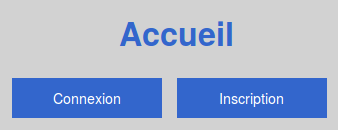
\includegraphics[scale=0.5]{../graph/1-accueil.png} 
  \end{figure}
    
    \subsection{Inscription}
    Après avoir cliqué sur le bouton \textbf{Inscription}, la formulaire suivant s'affiche :
    \begin{figure}[H]
      \center 
      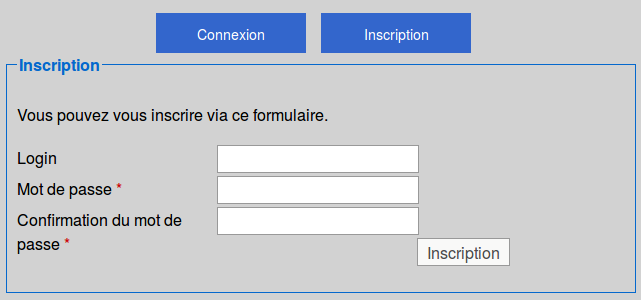
\includegraphics[scale=0.5]{../graph/2-inscription.png} 
    \end{figure}    
    Le joueur saisi alors son login et son mot de passe deux fois, sachant que s'il ne met pas deux fois le même mot de passe, ou s'il tente d'utiliser un login déjà existant un message d'erreur sera affiché (en rouge), sinon un message vert indiquera que l'inscription a bien été effectuée.
    \begin{figure}[H]
      \center 
      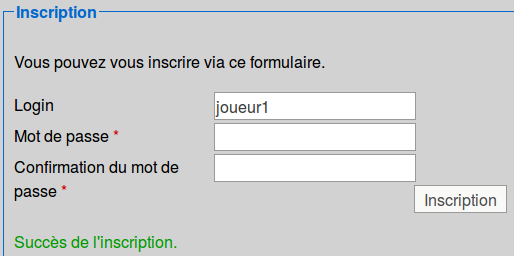
\includegraphics[scale=0.36]{../graph/2.1-inscriptionsucces.png} 
      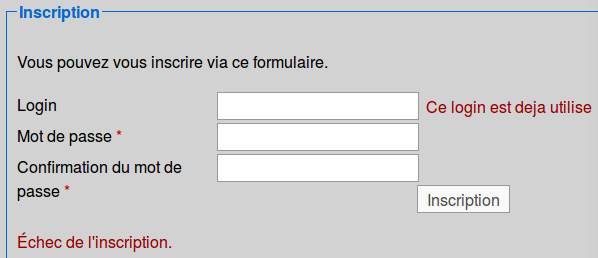
\includegraphics[scale=0.36]{../graph/2.2-inscriptionechec.png} 
    \end{figure}

    \subsection{Connexion}
    Maintenant que le joueur est inscrit, il peut se connecter via un autre formulaire où il lui ai demandé de saisir login et mot de passe (qui doivent toujours être valides). 
    \begin{figure}[H]
      \center
      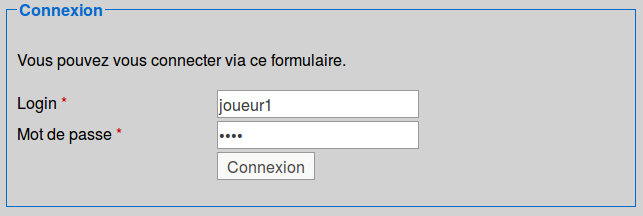
\includegraphics[scale=0.5]{../graph/3-connexion.png}
    \end{figure}

  \section{Joueur connecté}  
  Après avoir validé son formulaire de connexion, et si les identifiants ont bien été saisis, l'application va télécharger les historiques des cours non présents dans la base de données.\\
  
  \noindent Le chargement peut donc être assez long si c'est la première connexion ou si cela fait longtemps qu'on ne s'est pas connecté.\\
  
  \noindent Le joueur arrive ensuite sur une nouvelle page d'accueil dans laquelle on visulalise un menu horizontal ainsi que deux boutons : l'un permettant d'aller vers son \textbf{portefeuille}, et l'autre vers la \textbf{bourse}.
  \begin{figure}[H]
    \center
    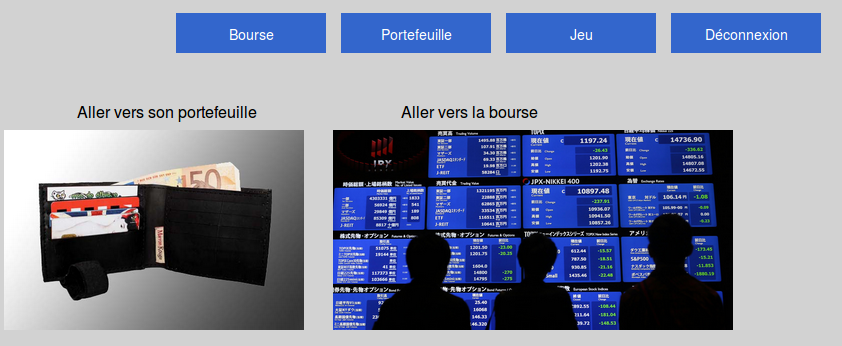
\includegraphics[scale=0.5]{../graph/4-accueilconnecte.png}
  \end{figure}
    
    \newpage
    \subsection{Bourse}
    Prenons le cas où il décide de consulter la \textbf{bourse}, ou plutôt l'échantillon de la bourse que le broker propose à ses clients. Dans un premier temps, le joueur arrive sur la page suivante (vide et une simple barre de recherche) : 
    \begin{figure}[H]
      \center
      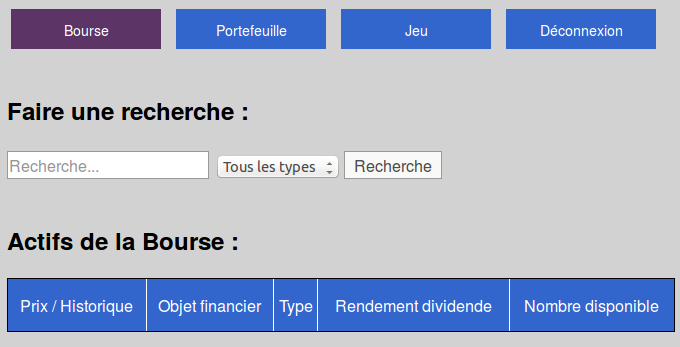
\includegraphics[scale=0.4]{../graph/5-accueilbourse.png}  
    \end{figure}
      
      \begin{enumerate}
       \item \textbf{Recherche :} le joueur peut effectuer une recherche par mot clés et/ou par type d'actif financier. Par exemple, l'utilisateur peut saisir 'app' et choisir 'Action' en espérant obtenir l'action de la société Apple (si elle existe dans l'échantillon). La recherche s'effectue et on voit s'afficher toutes les \textbf{actions} ayant les lettres 'aap' (peu importe la casse) dans le libellé ou dans le code. On voit alors le résultat de la recherche qui se compose de 3 actions avec le détail de celles-ci. 
      \begin{figure}[H]
	\center
	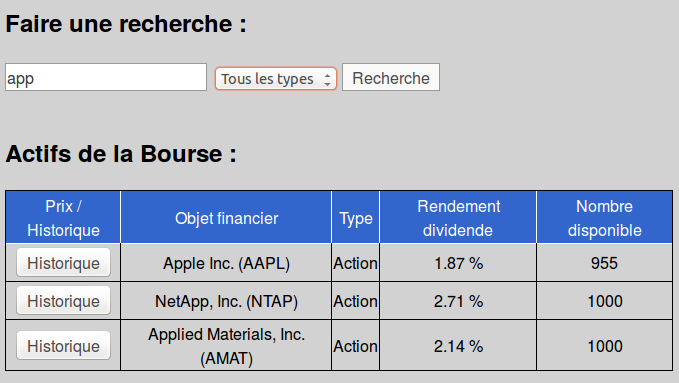
\includegraphics[scale=0.5]{../graph/5-rechercheactifs.png}
      \end{figure}
      
      \newpage
      La même chose peut s'effectuer sur une recherche sans mot clé et seulement sur les obligations :
      \begin{figure}[H]
	\center      
	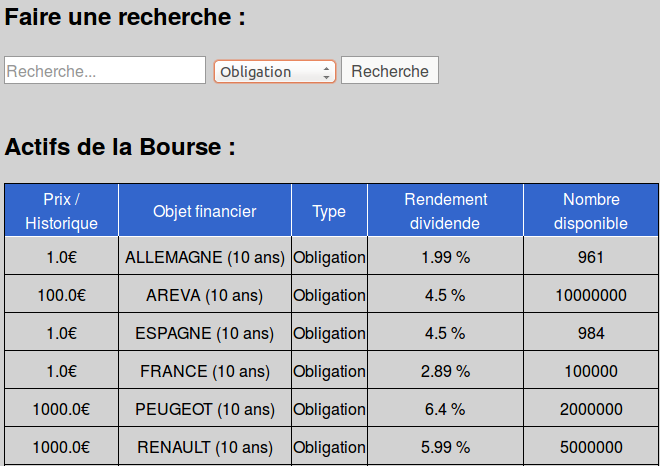
\includegraphics[scale=0.5]{../graph/5-rechercheobligations.png}
      \end{figure}
      
      On suppose finalement que la recherche abouti au résultat suivant et que le joueur souhaite en savoir plus sur cette action et clique sur le bouton \textbf{Historique}.
      \begin{figure}[H]
	\center      
	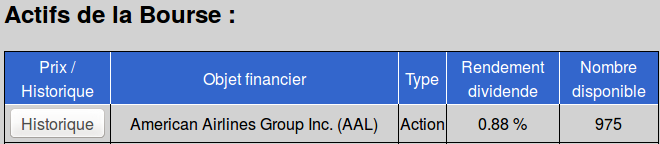
\includegraphics[scale=0.5]{../graph/5-detailaction.png}
      \end{figure}
      
      \item \textbf{Historique :} le joueur peut accéder à l'historique des actions et des indices. Ceux-ci ont été récupérés par l'application sur Yahoo! Finance et sont mis à disposition des joueurs sous différentes formes. La première est simplement sous forme d'un tableau de valeurs classé par dates.
      \begin{figure}[H]
	\center
	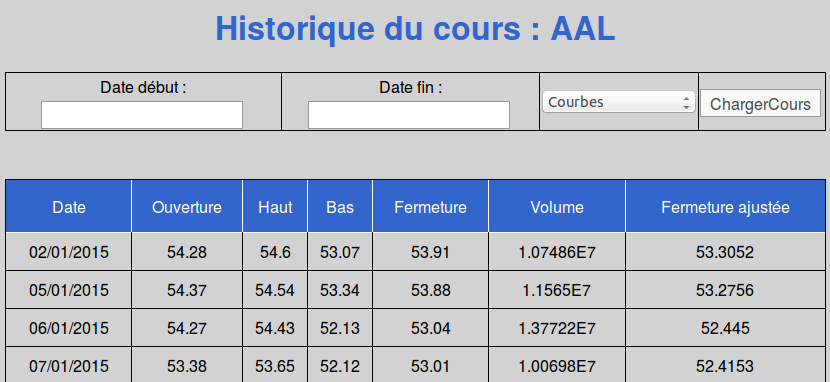
\includegraphics[scale=0.5]{../graph/6-historiquetableau.png}
      \end{figure}
      
      A propos de dates justement, il est possible de choisir l'intervalle de temps que l'on souhaite observer grâce à des calendriers qui sont affichés grâce à une fonction JavaScript :
      \begin{figure}[H]
	\center
	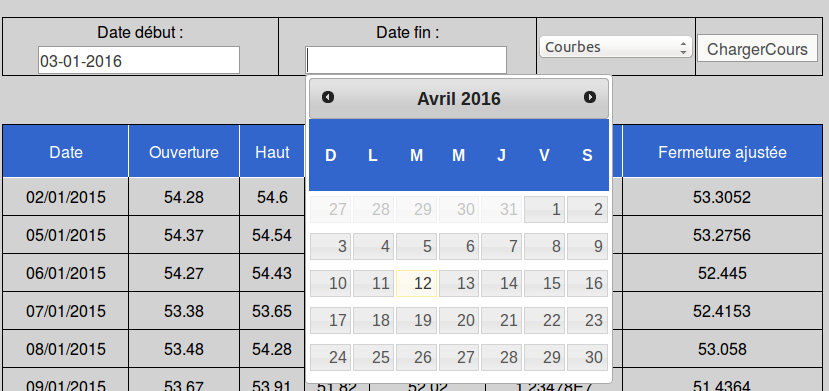
\includegraphics[scale=0.5]{../graph/6-recherchecalendrier.png}
      \end{figure}
      
      Il est également possible de sélectionner le type d'affichage d'historique que l'on souhaite. Nous avons choisi de proposer cinq indicateurs différents : 
      \begin{enumerate}
	\item une courbe simple de l'historique du cours :
	  \begin{figure}[H]
	    \center
	    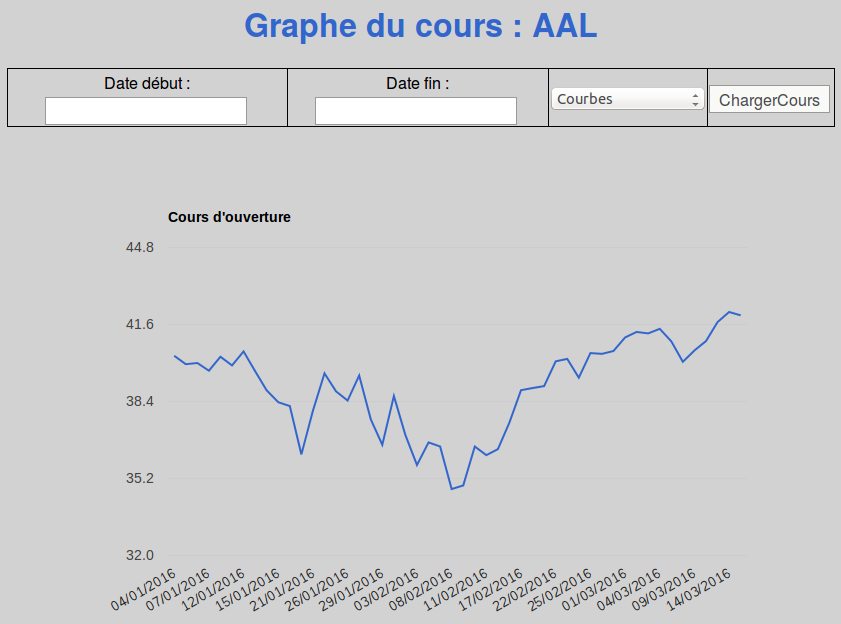
\includegraphics[scale=0.5]{../graph/6-historiquecourbe.png}
	  \end{figure}
	\newpage  
	\item des chandeliers pour lequels il vaut mieux prendre un intervalle de temps réduit pour bien les visualiser : 
	  \begin{figure}[H]
	    \center
	    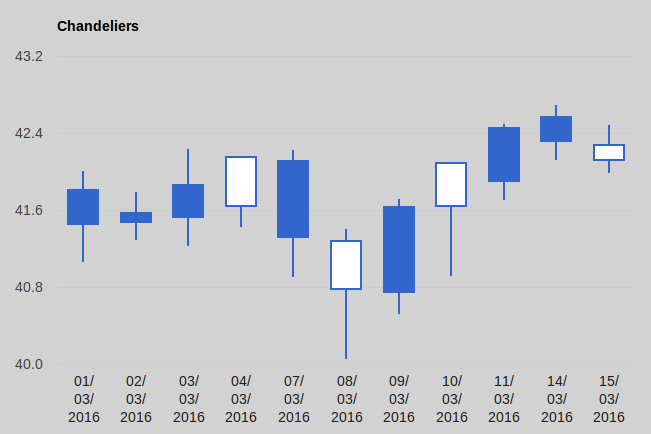
\includegraphics[scale=0.5]{../graph/6-historiquechandeliers.png}
	  \end{figure}
	\item les volumes échangés chaque jours sous forme de diagramme en barre :
	  \begin{figure}[H]
	    \center
	    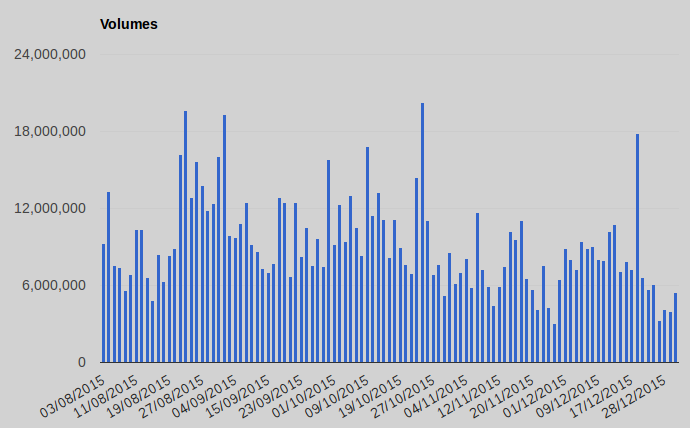
\includegraphics[scale=0.5]{../graph/6-historiquevolumes.png}
	  \end{figure}
	\newpage  
	\item la moyenne mobile à deux jours (ici mieux vaut une période assez longue) :
	  \begin{figure}[H]
	    \center
	    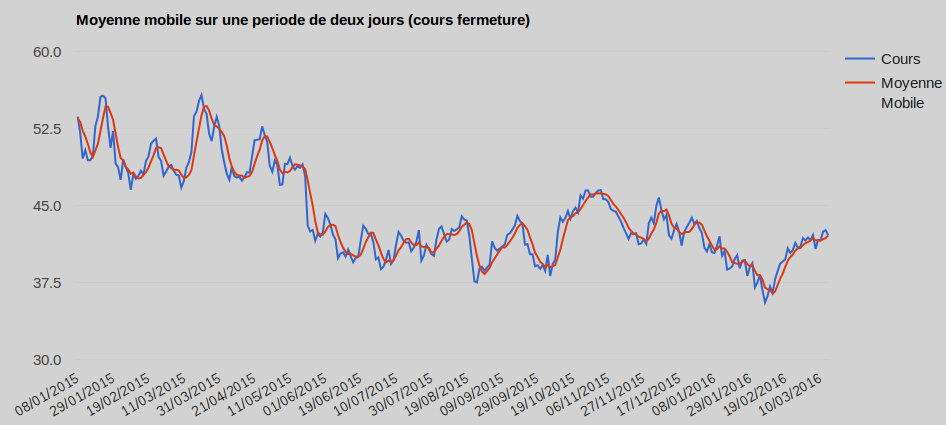
\includegraphics[scale=0.5]{../graph/6-historiqueMoyMob.png}
	  \end{figure}
	\item les bandes de Bollinger (période longue également) :
	  \begin{figure}[H]
	    \center
	    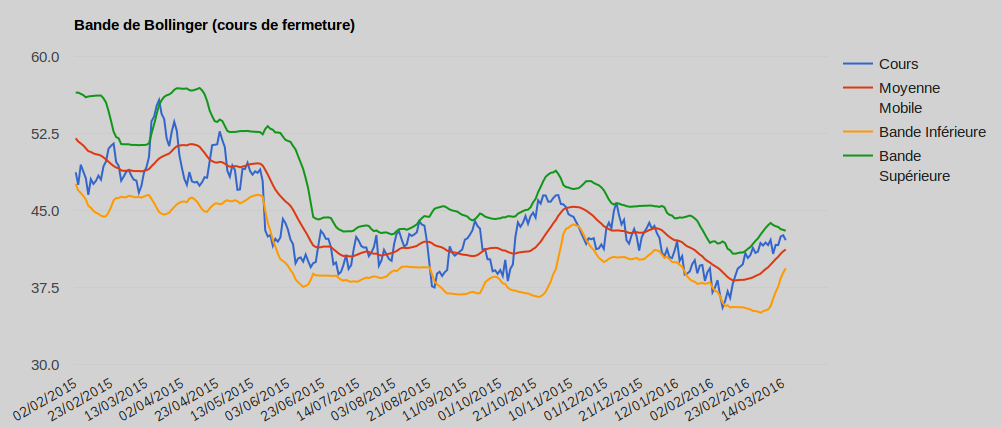
\includegraphics[scale=0.5]{../graph/6-historiqueBollinger.png} 
	  \end{figure}
      \end{enumerate}
      Tous ces graphiques ont pu être tracé grâce à l'API Google Chart, il est donc nécessaire d'être connecté à Internet pour les observer.
      
      \end{enumerate}
    
    \subsection{Portefeuille}
    La deuxième partie importante de notre application concerne le portefeuille d'actifs financiers et sa gestion. Il est possible via notre site Web, d'achat et vendre des actifs mais également d'accéder à une page donnant des chiffres clés sur le portefeuille constitué par le joueur. Lorsque l'on clique sur le menu portefeuille on atteint la page suivante (qui dans ce cas est vide car il n'y a pas encore d'actifs dans le portefeuille) :\\
    \begin{figure}[H]
      \center
      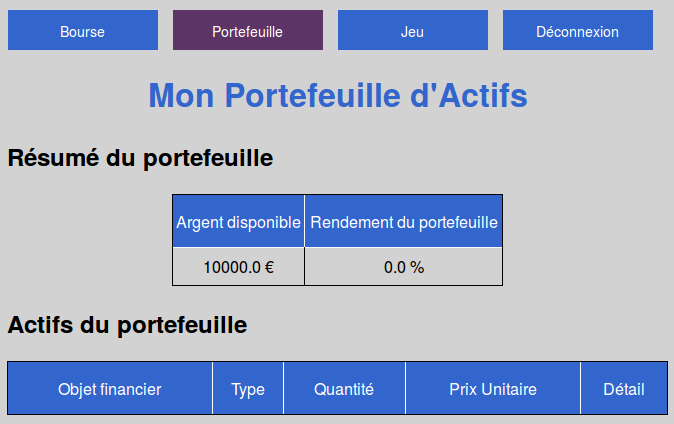
\includegraphics[scale=0.5]{../graph/7-accueilportefeuillevide.png}
    \end{figure}
    On observe sur cette page la quantité d'argent disponible au sein du portefeuille, le rendement de celui-ci, et quand il y en a la liste des actifs possédés.
      
      \begin{enumerate}
       \item \textbf{Achat d'actifs financiers :} dans un premier temps, nous allons acheter des actifs financiers. Nous disposons au départ de 10000€. Après avoir effectuer une recherche via la page \textbf{Achat} dans l'onglet \textbf{Portefeuille} on obtient un liste d'actions par exemple. On souhaite acheter 15 actions \textit{American Airlines Group Inc.} à 42.11€ l'unité. On clique alors sur le bouton acheter.
      \begin{figure}[H]
	\center
	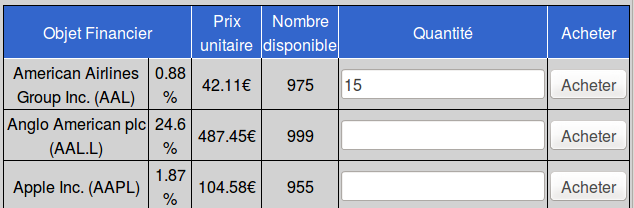
\includegraphics[scale=0.5]{../graph/7-achataction.png}
      \end{figure}

      On souhaite ensuite acheter une \textbf{Obligation} étatique par exemple, on choisit l'Espagne, la durée de l'emprunt fait par le pays est de 10ans (c'est un choix de notre part qui a été fixé pour toutes les obligations). Le prix unitaire est de 1€ et la quantité 60.
      \begin{figure}[H]
	\center
	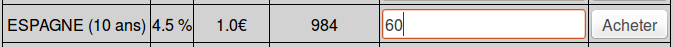
\includegraphics[scale=0.5]{../graph/7-achatobligation.png}
      \end{figure}
      
      L'exemple suivant va nous montrer que le système gère également les achats irréalisables. Par exemple, si on tente d'acheter 1 \textbf{Indice} du \textit{Dow Jones} à 17251.5€ l'unité, cela est impossible (puisque nous disposons de moins de 10000€ après les achats précédents) :
      \begin{figure}[H]
	\center
	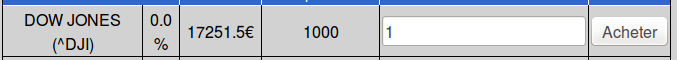
\includegraphics[scale=0.5]{../graph/7-achatindicetropcher.png}
      \end{figure}
      
      \newpage
      Le message d'erreur suivant est alors affiché et l'achat n'a pas été effectué :
      \begin{figure}[H]
	\center
	
\includegraphics[scale=0.5]{../graph/7-achatindiceechec.png}
      \end{figure}
     
      En revanche, à chaque fois qu'un achat a pu être effectué, le joueur est redirigé vers la page d'accueil du portefeuille comme suit (on observe bien les actifs qui ont été achetés et une action supplémentaire \textit{ALV.DE} acheté également) :
      \begin{figure}[H]
	\center
	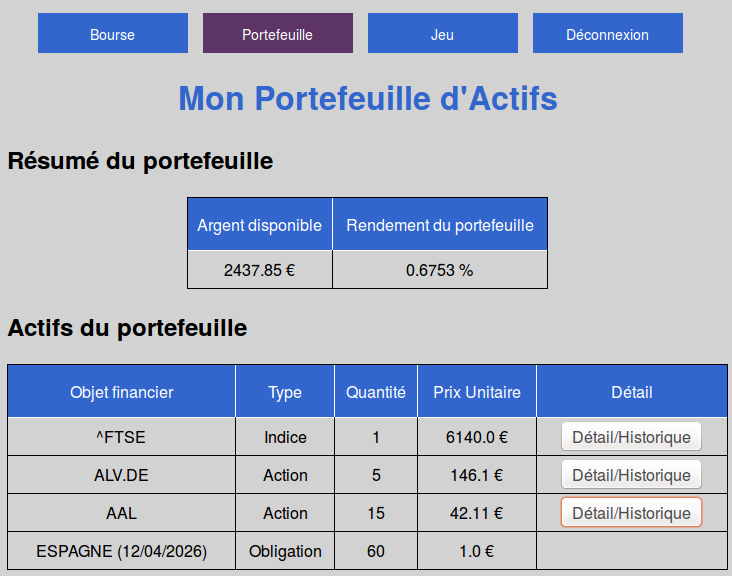
\includegraphics[scale=0.5]{../graph/7-vueportefeuilleapresachats.png}
      \end{figure}
      Une autre remarque sur cette page concerne le rendement du portefeuille. Celui-ci a été recalculé à chaque nouvel achat d'actif. De plus, le prix unitaire de chaque actif au sein du portefeuille est la somme pondéré des prix à chaque achat de cet actif (par exemple, si dans deux jours on rachète le même actif, le prix unitaire vaudra la moyenne pondérée par la quantité achetée aujourd'hui et celle achetée dans deux jours).
      
      \item \textbf{Vente d'actifs financiers :} l'étape suivante est la vente d'actifs financiers possédés par le joueur. Pour cela, il faut se rendre dans l'onglet \textbf{Vente} du menu \textbf{Portefeuille}. On atteint alors la page suivante :
      \begin{figure}[H]
	\center
	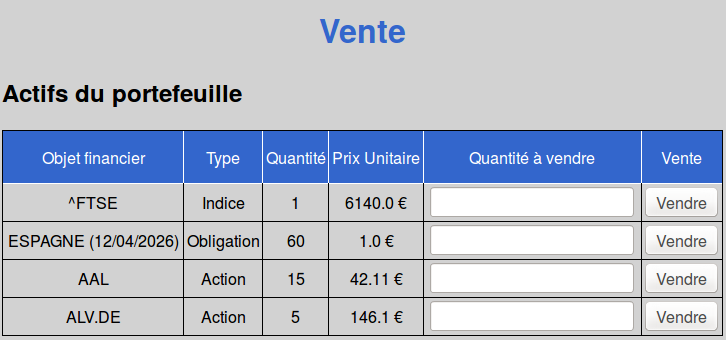
\includegraphics[scale=0.5]{../graph/7-vente.png}
      \end{figure}
      
      Imaginons que l'on souhaite vendre 1 \textbf{Action} \textit{AAL}. On saisi la quantité dans la case correspondante et on appuie sur le bouton vente de la même ligne :
      \begin{figure}[H]
	\center
	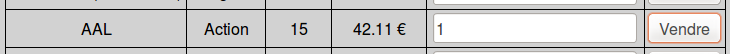
\includegraphics[scale=0.5]{../graph/7-vente1action.png}
      \end{figure}
      
      Suite à la vente, le joueur est redirigé vers la page d'accueil du portefeuille si la vente a bien été effectuée, sinon il reçoit un message d'erreur (dans le cas où il essaye de vendre plus que ce qu'il possède) :
      \begin{figure}[H]
	\center
	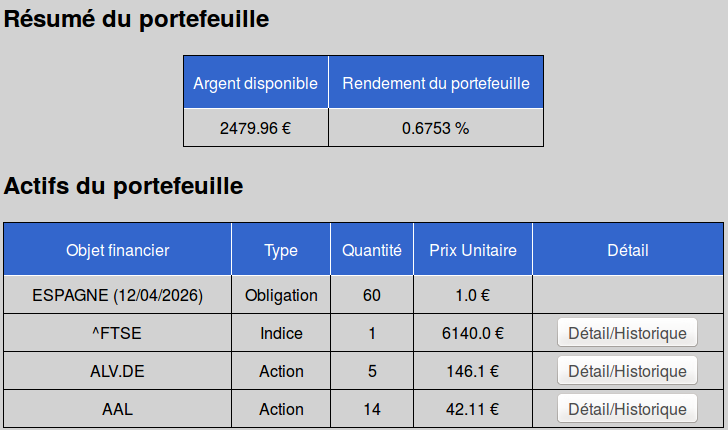
\includegraphics[scale=0.5]{../graph/7-accueilapresvente.png}
      \end{figure}
      Sur cette même page, on peut voir qu'il y a un bouton \textbf{Détail/Historique} qui permet de voir des détails sur les actions ou les indices. Via ce bouton, on accède à la même page que vu précédemment dans la partie \textbf{Historique}.
	
      \item \textbf{Indicateurs :} en parralèlle de l'achat et la vente d'actifs, il est possible d'obtenir quelques indicateurs sur le portefeuille dans sa globalité. C'est l'onglet \textbf{Indicateurs} du menu portefeuille qui permet d'y aller. Nous proposons différents indicateurs :
      \begin{enumerate}
       \item Les camemberts : ils permettent de voir la répartition du portefeuille selon la quantité de chaque type d'actifs financiers ou selon la somme d'argent investie dans chaque type. Cela peut être utile si l'on souhaite s'interroger sur la \textbf{diversification} du portefeuille.
	  \begin{figure}[H]
	    \center
	    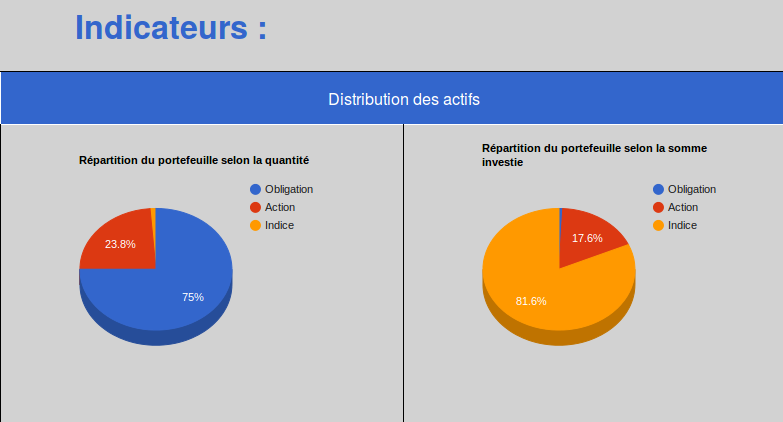
\includegraphics[scale=0.5]{../graph/7-indicateursPtfcamemberts.png}
	  \end{figure}
	  
       \item Les courbes des actions et indices en base 100 : cela permet de visualiser les historiques des actions et indices du portefeuille sur une période. On peut voir par exemple si les actifs sont corrélés ou pas.
	  \begin{figure}[H]
	    \center
	    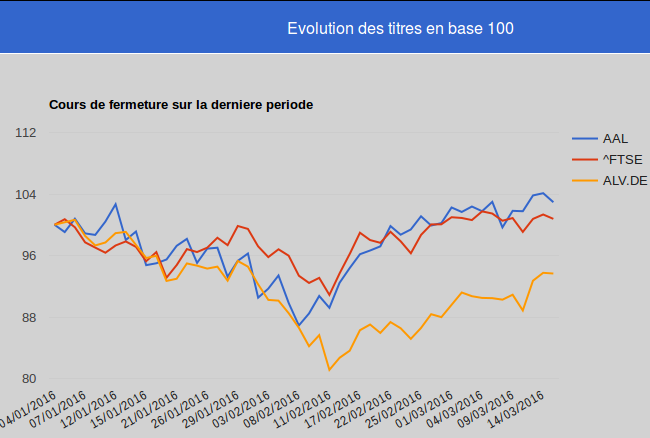
\includegraphics[scale=0.5]{../graph/7-indicateursbase100.png}
	  \end{figure}
      
      \end{enumerate}

      \item \textbf{Exporter :} afin d'obtenir d'autres indicateurs tels que la meilleure distrubition du portefeuille avec la méthode de Markowitz, nous avons mis à disposition une page permettant d'exporter le portefeuille au format \textbf{.csv}. Il faut copier-coller le texte de la page Web visible lorsque l'on clique sur l'onglet \textbf{Exporter}. Dans ce fichier qui résume le portefeuille depuis sa création on a accès à :
      \begin{itemize}
       \item L'argent non investi disponible
       \item La composition actuelle du portefeuille
       \item L'historique des actions (achat/vente) qui ont été effectuées
       \item L'espérance des rendements de chaques indices et actions
       \item La matrice de covariance des rendements
      \end{itemize}

      \begin{figure}[H]
	\center	
	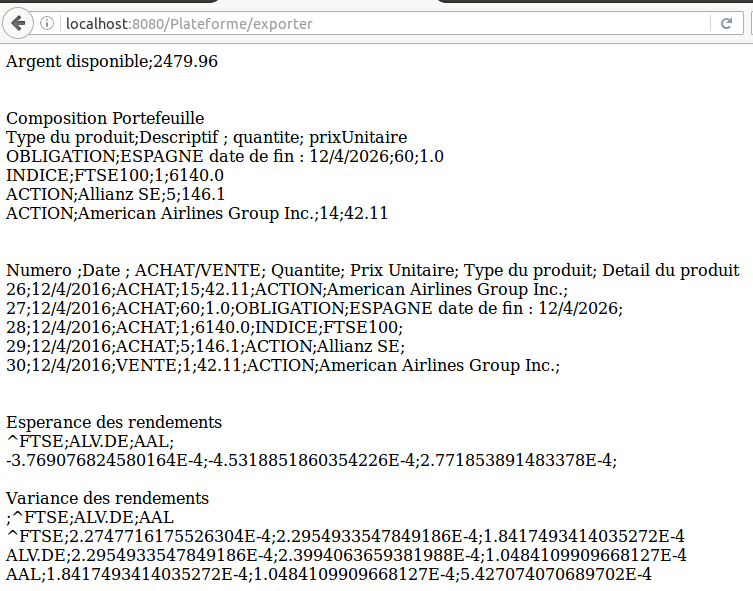
\includegraphics[scale=0.5]{../graph/7-exporterpage.png}
      \end{figure}

    \end{enumerate}
  
    \subsection{Jeu}
    Le dernier menu auquel on peut accéder concerne le jeu en cours. On considère que chaque joueur à un portefeuille et on classe les joueurs selon l'argent qu'ils possèdent (ils ont le même argent disponible au départ). Pour faire le classement, on fait la somme des prix actuels des actifs multipliées par la quantité correspondante et on ajoute l'argent disponible. Il est également possile d'abandonner la partie si l'on considère que les choix on été trop mauvais et repartir de zéro en ayant un nouveau portefeuille.
  
    \begin{enumerate}
     \item \textbf{Le classement :} on affiche les différents joueurs et leur score. Le joueur courant (celui qui est connecté) et en rouge :
     \begin{figure}[H]
	\center
	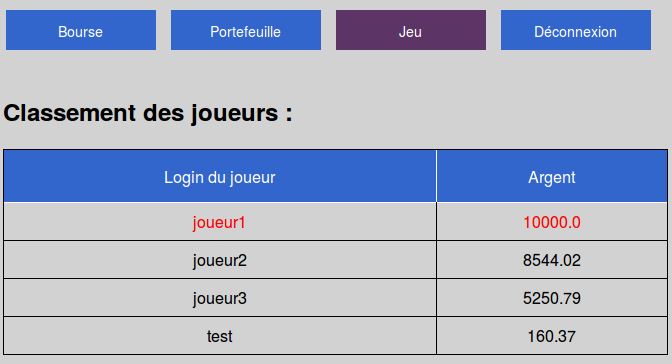
\includegraphics[scale=0.5]{../graph/8-jeuclassement.png}
      \end{figure} 
     \item \textbf{La réinitialisation :} tout le portefeuille est remis à zéro, le joueur possède à nouveau 10000€.
      \begin{figure}[H]
	\center
	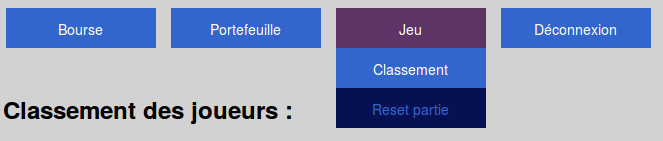
\includegraphics[scale=0.5]{../graph/8-jeuresetpartie.png}
      \end{figure} 
    \end{enumerate}
  
    \subsection{Déconnexion}
    La dernière étape avant de fermer l'application est de se déconnecter. On est alors redirigé vers la page d'accueil vu au début.